Los autores, José Santos y Ángel Monteagudo, decidieron utilizar un autómata celular
siguiendo un modelo de eventos. Es decir, por un lado, la simulación se realiza
sobre una rejilla en tres dimensiones, comenzando con una única célula en el centro de la misma.
Por otro lado, se programan una serie de eventos para cada una de las células de la rejilla, aleatoriamente
entre 5 y 10 (ambos inclusive) iteraciones en el futuro.

Las características y propiedades del sistema se describen en las secciones de este capítulo que
se muestran a continuación.

\section{Objetivos del artículo}

En este trabajo, los autores tiene como objetivo estudiar las fases iniciales del crecimiento tumoral a nivel celular,
estudiando diferentes configuraciones iniciales y observando las diferentes dinámicas y comportamientos. Así como,
estudiar, también, la relevancia en la progresión del cáncer de cada uno de los marcadores, y qué
dinámicas presenta cada uno de ellos.

Además, centran el foco de su trabajo en las transiciones cuando las células cancerosas
mueren con una probabilidad dada durante la progresión del sistema celular.

No son objetivos de este trabajo simular las fases posteriores al crecimiento inicial de tumores, ni el
aumento de tamaño de las células. Tampoco es objetivo modelar los diferentes factores que
pueden provocar mutaciones y/o muerte celular.

Por último, en este artículo no se presta atención a las células madre del cáncer. Los autores en
otros trabajos \cite{jsantos-amonteagudo-2015} sí modelizan la presencia de dichas células.

\section{Las células, genoma y propiedades}

Cada célula estará alojada en una única posición del autómata. En esta simulación, no se modeliza
el tamaño de las células, es decir, aunque en las células cancerosas se observa, además de un comportamiento
replicativo sin control, un crecimiento en su tamaño sin control, los autores no han tenido en cuenta esto.

Cada célula presente en la rejilla cuenta con un genoma y unas propiedades únicas para cada una de ellas.
En cuanto a su genoma, cuenta con 5 variables binarias que representan la presencia o no de hasta cinco mutaciones, las cuales, definen
un determinado comportamiento canceroso en cada caso. Estas mutaciones son las siguientes:

\begin{itemize}
    \item \textbf{SG}: Autogeneración de los mensajes de crecimiento. Esto es, la mutación que permite que la
    célula genere sus propios mensajes para ejecutar la división con independencia externa.
    \item \textbf{IGI}: Inhibición de las señales de anticrecimiento. Esto es, ante la recepción de una orden
    de detener su crecimiento, la célula tiene una mutación que le permite un mecanismo de ignorancia de los mismos.
    \item \textbf{EA}: Evasión de apoptosis. Esto es, la célula puede, mediante mutación, no hacer caso ante
    una orden de apoptosis, o muerte celular controlada.
    \item \textbf{EI}: Inmortalidad efectiva. Esto es, la célula adquiere una mutación que permite evitar un límite
    replicativo existente, entre otros factores, por el tamaño del telómero.
    \item \textbf{GI}: Inestabilidad genética. Esto es, una mutación que permite a la célula acumular más daño genético, es decir,
    la tasa de mutación base se va incrementando con el paso del tiempo.
\end{itemize}

Además, cada célula tiene una tasa de mutación base y un tamaño de telómero. El primero, es utilizado a la hora
de añadir nuevas mutaciones a la célula. Y la segunda, es un límite replicativo debido a que el ADN queda
desprotegido para futuras mutaciones y podrían ocurrir errores.

\section{Parámetros globales}

De cara a la simulación, existen una serie de parámetros globales que inciden en determinados mecanismos y,
por tanto, afectan en su evolución. Esto son:

\begin{itemize}
    \item \textbf{t}: Tamaño de la rejilla.
    \item \textbf{m}: Valor por defecto que indica la tasa de mutación base de cada célula al inicio.
    \item \textbf{tl}: Valor por defecto que indica el tamaño del telómero de cada célula al inicio.
    \item \textbf{e}: Valor por defecto utilizado para definir la probabilidad de una célula de morir por daño genético.
    \item \textbf{i}: Valor por defecto utilizado como factor de aumento de la tasa de mutación base de las células.
    \item \textbf{g}: Valor por defecto para ver qué probabilidad hay de que una célula cancerosa mate a un vecino para
    poder reproducirse.
    \item \textbf{a}: Valor por defecto para ver con qué probabilidad una célula muere de forma aleatoria. Este parámetro
    se introduce como forma de simular las muy diversas causas que pueden originar en la muerte de la célula, por ejemplo,
    recibir una alta dosis de radiación entre otras.
\end{itemize}

\section{Pruebas previas a la mitosis}

El modelo de eventos, a la hora de realizar la mitosis (división celular), realiza tres pruebas:

\begin{itemize}
    \item \textbf{Prueba de muerte aleatoria}: La célula muere con una probabilidad dada ($1/a$).
    \item \textbf{Prueba de daño genético}: A mayor cantidad de mutaciones, mayor probabilidad de
    que la célula muera ($n/e$, donde $n$ es el número de mutaciones de la célula). Excepto, que
    la célula tenga la mutación $EA$ presente en su genoma.
    \item \textbf{Prueba de mitosis}: En realidad, se trata de tres pruebas cuyo resultado debe
    ser positivo para que la célula pueda ejecutar la mitosis:
    \begin{itemize}
        \item \textbf{Comprobación del factor de crecimiento}: La célula sólo puede realizar la
        mitosis si se encuentra dentro de un límite espacial predefinido. Es decir, hay suficiente
        factor de crecimiento. Fuera de este área no podrá realizar la mitosis, excepto si el
        marcador $SG$ está activo.
        \item \textbf{Comprobación de ignorancia de inhibición de crecimiento}: Si no hay
        espacio en el vecindario, la célula no podrá realizar la división. Excepto, que
        la mutación $IGI$ esté presente, en cuyo caso, reemplazará a un vecino con una
        probabilidad dada ($1/g$).
        \item \textbf{Comprobación de potencial replicativo sin límites}: Si el tamaño del telómero
        es $0$, la célula muere. Excepto si el marcador $EI$ está presente.
    \end{itemize}
\end{itemize}

En estas pruebas, se utilizan los parámetros globales, además, de las propiedades y el genoma de la célula.

Por tanto, si una célula pasa todas las pruebas podrá entrar en fase de mitosis.

\section{Mitosis}

La mitosis es la fase donde se realiza la división celular, lo cual origina una nueva célula, llamada
célula hija, que es una copia exacta de la célula original.

Durante este proceso, se pueden producir una serie de errores, bien de forma natural, o bien, debido
mutaciones presentes en la célula original que hacen más probable un error.

En este trabajo, el proceso de mitosis cuenta con los siguientes pasos:

\begin{itemize}
    \item Incremento de la tasa de mutación base $m$ (de acuerdo al parámetro global $i$) si el marcador
    $GI$ está presente.
    \item Añadir nuevas mutaciones a la célula de acuerdo a la tasa base de mutación ($1/m$).
    \item Decrementar el telómero en ambas células en una unidad, siempre que su tamaño no sea 0.
\end{itemize}

A continuación, se describe como se programan nuevos eventos mitóticos para ambas hijas.

\section{Eventos mitóticos}

Un evento mitótico se puede ver como la posibilidad de que una célula ejecute o no la división (o mitosis),
en el futuro.

Todas las células en la rejilla contarán con un evento mitótico en el futuro. Cuando se selecciona una
de las candidatas en cada iteración la célula candidata debe pasar las pruebas previas a la mitosis para ver
si la misma puede o no ejecutar la mitosis. Si el resultado es positivo, se realiza la mitosis y se crean
nuevos eventos mitóticos en el futuro para la célula original y, también, para la célula hija.
Si el resultado es negativo, pero la célula no ha muerto, se programa un nuevo evento mitótico en el futuro.

La programación de eventos mitóticos futuros consiste en la generación, de forma aleatoria, de un valor
entre $5$ y $10$ iteraciones (ambas inclusive) del bucle principal. Estos valores tienen que ver con el ciclo de vida
temporal de las células, sobre el cual, se detalla más información en la siguiente sección.

\section{Equivalencia temporal}

El ciclo de vida de las células biológicas es de entre $15$ y $24$ horas. Este ciclo se divide en $5$ fases, que son:
fase $G0$, fase $G1$, fase $S$, fase $G2$ y fase $M$.

Una célula parte en fase de reposo ($G0$). Si hay espacio suficiente a su alrededor (vecindario) automáticamente pasa
a fase $G1$. En la simulación, $G1$ se simula mediante el paso del tiempo (iteraciones) y la programación de
eventos mitóticos en el futuro (entre $5$ y $10$ iteraciones, ambas inclusive). Además, en la simulación no se
tiene en cuenta el crecimiento celular.

La fase $S$ es cuando tiene lugar la replicación del $ADN$. La cual, puede introducir una mutación ocasionalmente.
La célula entra en una última fase previa a la mitosis, llamada fase $G2$, en la cual se producen una serie
de comprobaciones sobre el daño genético. Esto, puede provocar la apoptosis (muerte celular programada) en la célula.

Finalmente, la célula entra en la fase $M$ o de mitosis. Todo este ciclo, que en la simulación toma entre $5$ y $10$ iteraciones
($15$ y $24$ horas en células biológicas) da una media de $2,6$ horas por iteración. Por ejemplo, para $5000$ iteraciones se tienen
unas $77,4$ semanas aproximadamente.

\section{Bucle principal del modelo de eventos}

El modelo de eventos consiste en realizar un número de iteraciones, y en cada iteración realizar
una serie de pruebas con aquellas células que tienen una posibilidad de evento mitótico en ese
momento, como se describe en la figura ~\ref{fig:eventmodel}.

Se realizan tres pruebas, la primera prueba consiste en comprobar si a la célula que tiene
un posible evento mitótico en esta iteración aplica o no muerte aleatoria. Esto se realiza mediante un
sorteo con una probabilidad dada ($1/a$). Mediante esta prueba se pretende simular las diferentes
causas que pueden llevar a la muerte de una célula.

En la segunda prueba, se pretende simular los mecanismos del cuerpo que evitan que una célula
siga reproduciéndose con un elevado daño genético. Esto se realiza mediante un sorteo con una probabilidad
dada ($n/e$) a partir del número de mutaciones de la célula entre un parámetro global establecido para
la simulación.

Y, por último, se realiza la prueba para ver si dicha célula realiza o no la mitosis.
Para ello, se realizan tres pruebas que deben ser positivas, estas son: comprobación del factor de crecimiento,
comprobación de ignorancia de inhibición de crecimiento, y comprobación de potencial replicativo sin límites.

\begin{figure}[h]
\centering
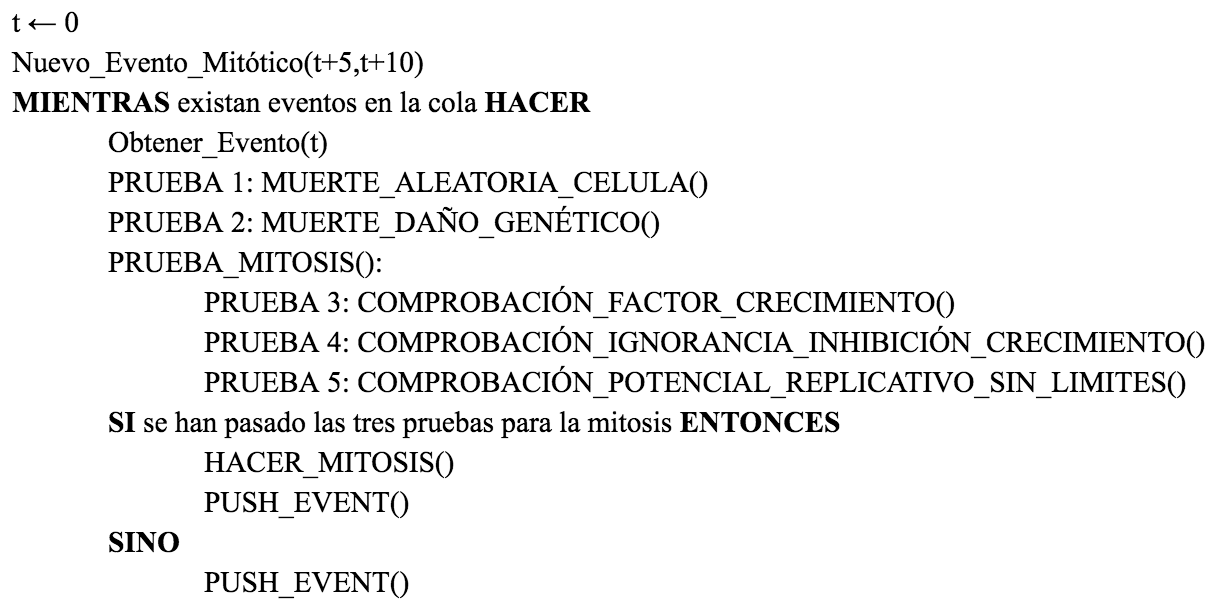
\includegraphics[scale=0.8]{figures/pseudo_alg}
\caption{Modelo de eventos para simulación del cáncer.}
\label{fig:eventmodel}
\end{figure}

La prueba número tres, o comprobación del factor de crecimiento, consiste en comprobar
si la célula está dentro de un espacio predefinido en el cual llegan los mensajes
para poder realizar la mitosis, y si no es así, se comprueba que tiene la mutación $SG$
que le permite realizar la mitosis a pesar de estar en dicha posición. En cuanto a la prueba
número cuatro, o comprobación de ignorancia de inhibición de crecimiento, consiste en comprobar
si hay espacio en el vecindario para realizar la mitosis, o en caso contrario, si tiene el marcador
$IGI$ reemplazará a un vecino con una probabilidad dada ($1/g$) mediante la muerte del vecino elegido.
Por último, la prueba número cinco, o comprobación de potencial replicativo sin limites,
consiste en comprobar si el tamaño del telómero es mayor a cero, o en caso contrario,
si tiene la mutación $EI$ que le permite realizar la mitosis a pesar de no contar con telómero.

Si la célula pasa todas las pruebas se procede a realizar la mitosis y a programar un nuevo evento mitótico para ambas.
En otro caso, se programa un nuevo evento mitótico para la misma célula si esta no ha muerto como
resultado de alguno de las pruebas previas a la mitosis.

La implementación final en un lenguaje de programación de propósito general varía dada
la complejidad de implementación de las pruebas descritas. En el siguiente capítulo se comenta y se muestra
la implementación final del algoritmo presentado en esta sección.
